\documentclass{article}     %
\usepackage[utf8]{inputenc} %
\usepackage[russian]{babel} %
\usepackage[OT1]{fontenc}   %

%\documentclass[a4paper]{jacow}
\usepackage{mathtools}
\usepackage{amsmath}
\usepackage{xfrac}
\usepackage{xparse}
\usepackage{subcaption}
\usepackage{graphicx}
\usepackage{url}
\usepackage{paralist}

\let\oldvec\vec
\renewcommand{\vec}{\boldsymbol}
\DeclareDocumentCommand{\bkt}{sm}{\IfBooleanTF{#1}{\left[ #2 \right]}{\left(#2\right)}}
\DeclareDocumentCommand{\ddt}{m}{\frac{\mathrm{d} {#1}}{\mathrm{d} t}}
\DeclareDocumentCommand{\pddx}{mO{t}O{}}{\frac{\partial^{#3} {#1}}{\partial {#2}^{#3}}}
\newcommand{\w}{\omega}
\newcommand{\W}{\Omega}
\newcommand{\avg}[1]{\langle {#1} \rangle}


\begin{document}

\begin{figure}[h]
  \centering
  \begin{subfigure}{\linewidth}
    \centering
    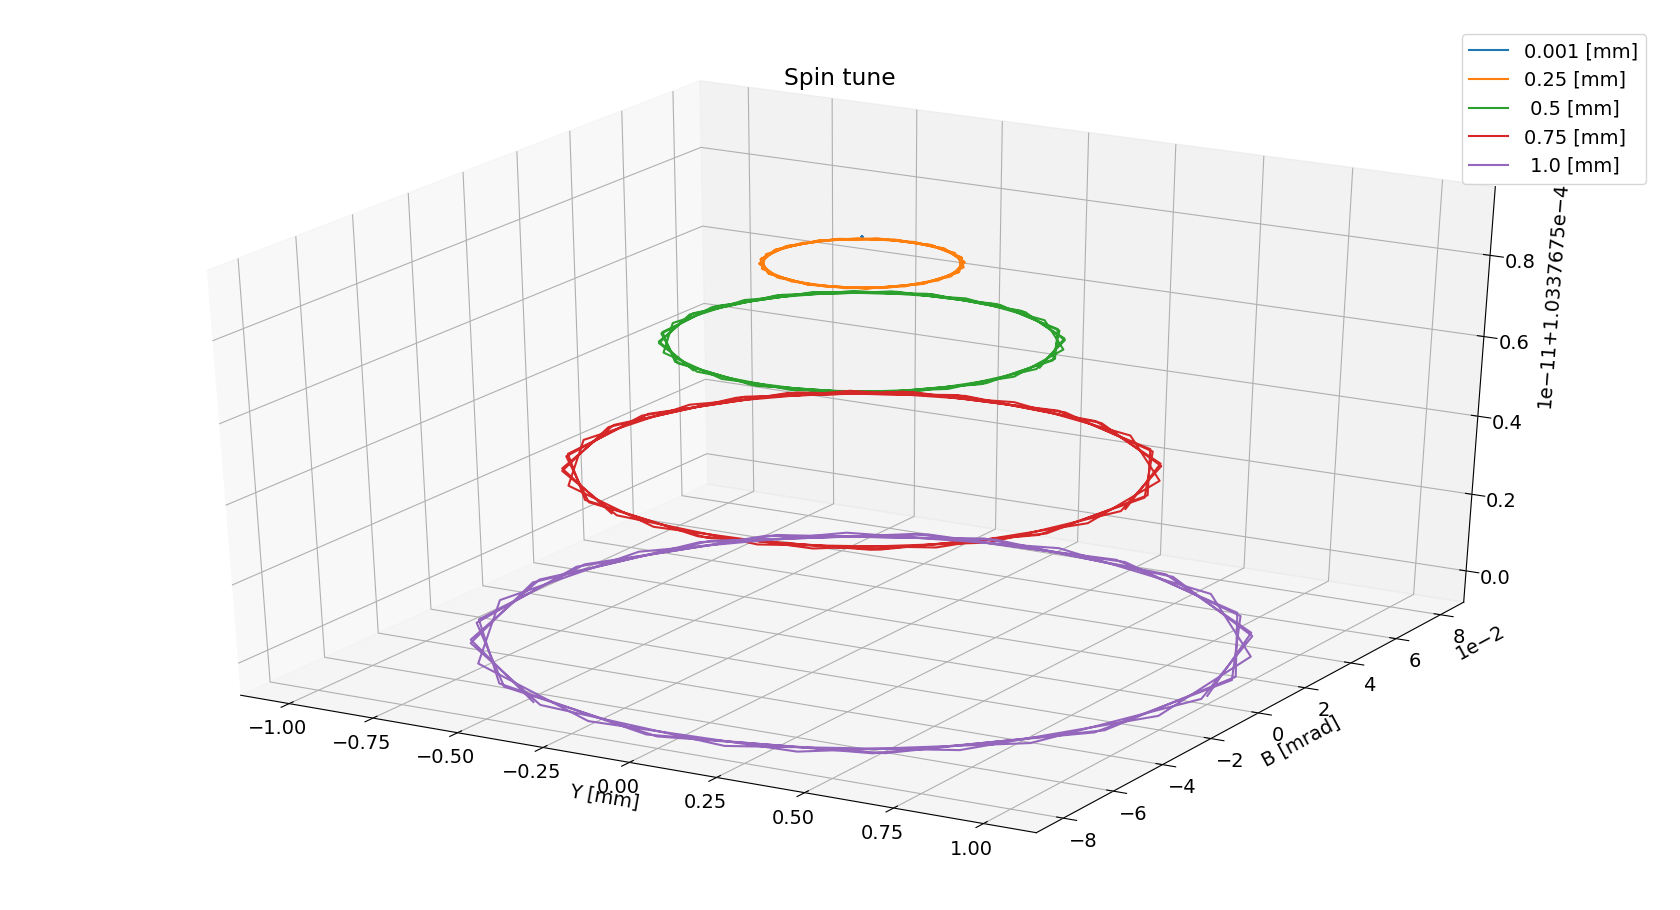
\includegraphics[width=\linewidth]{../img/IPAC19/ST_VS_YB_IMPERFECT_UNOPT}
    \caption{Не используя секступоли}
  \end{subfigure}
  \begin{subfigure}{\linewidth}
    \centering
    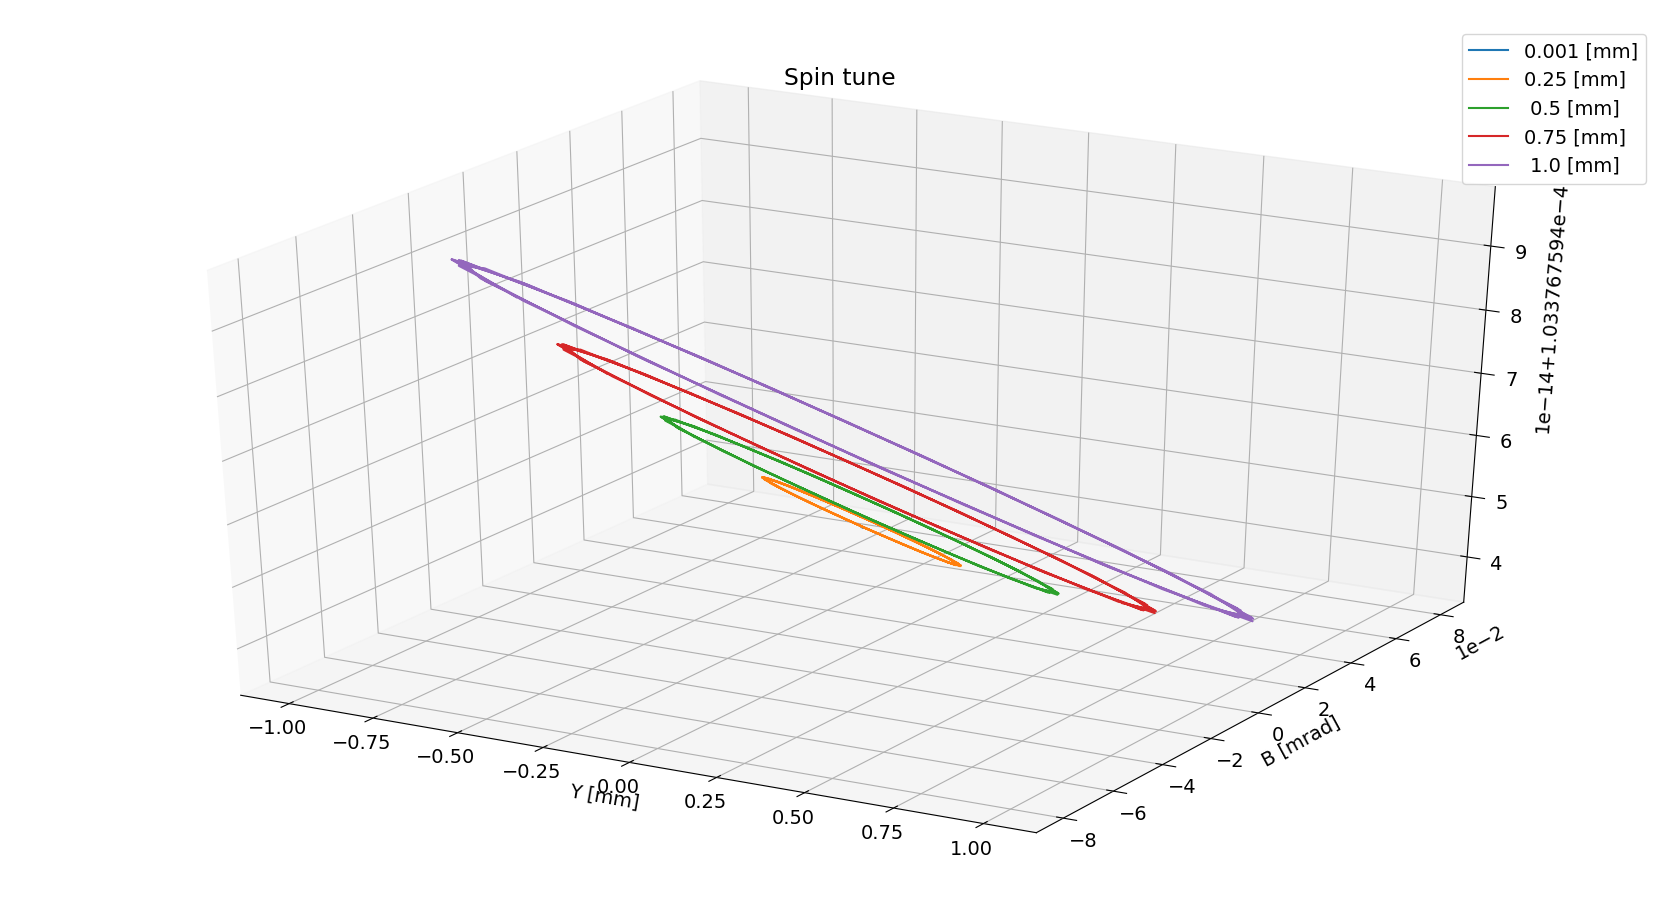
\includegraphics[width=\linewidth]{../img/IPAC19/ST_VS_YB_IMPERFECT_OPTIM}
    \caption{Используя секступоли\label{fig:spin_tune_optim}}
  \end{subfigure}
  \caption{Спин-тюн в имперфектной структуре как функция координаты
    фазового пространства $(y, y')$\label{fig:spin_tune}}
\end{figure}

\begin{figure}[h]
  \centering
  \begin{subfigure}{\linewidth}
    \centering
    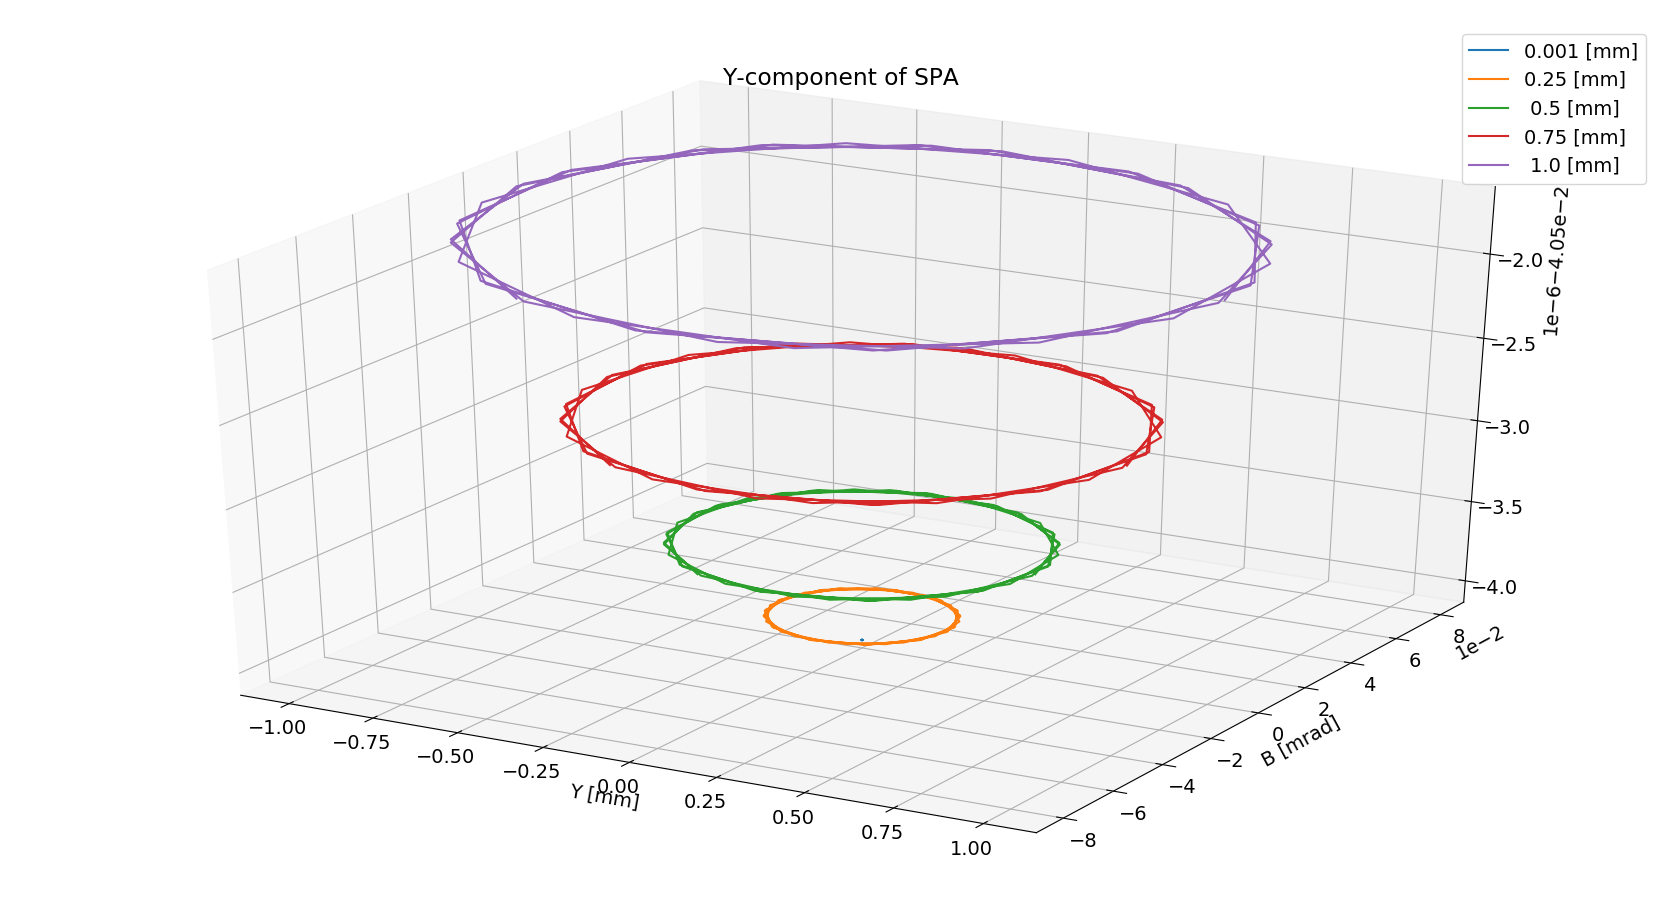
\includegraphics[width=\linewidth]{../img/IPAC19/NY_VS_YB_IMPERFECT_UNOPT}
    \caption{Не используя секступоли}
  \end{subfigure}
  \begin{subfigure}{\linewidth}
    \centering
    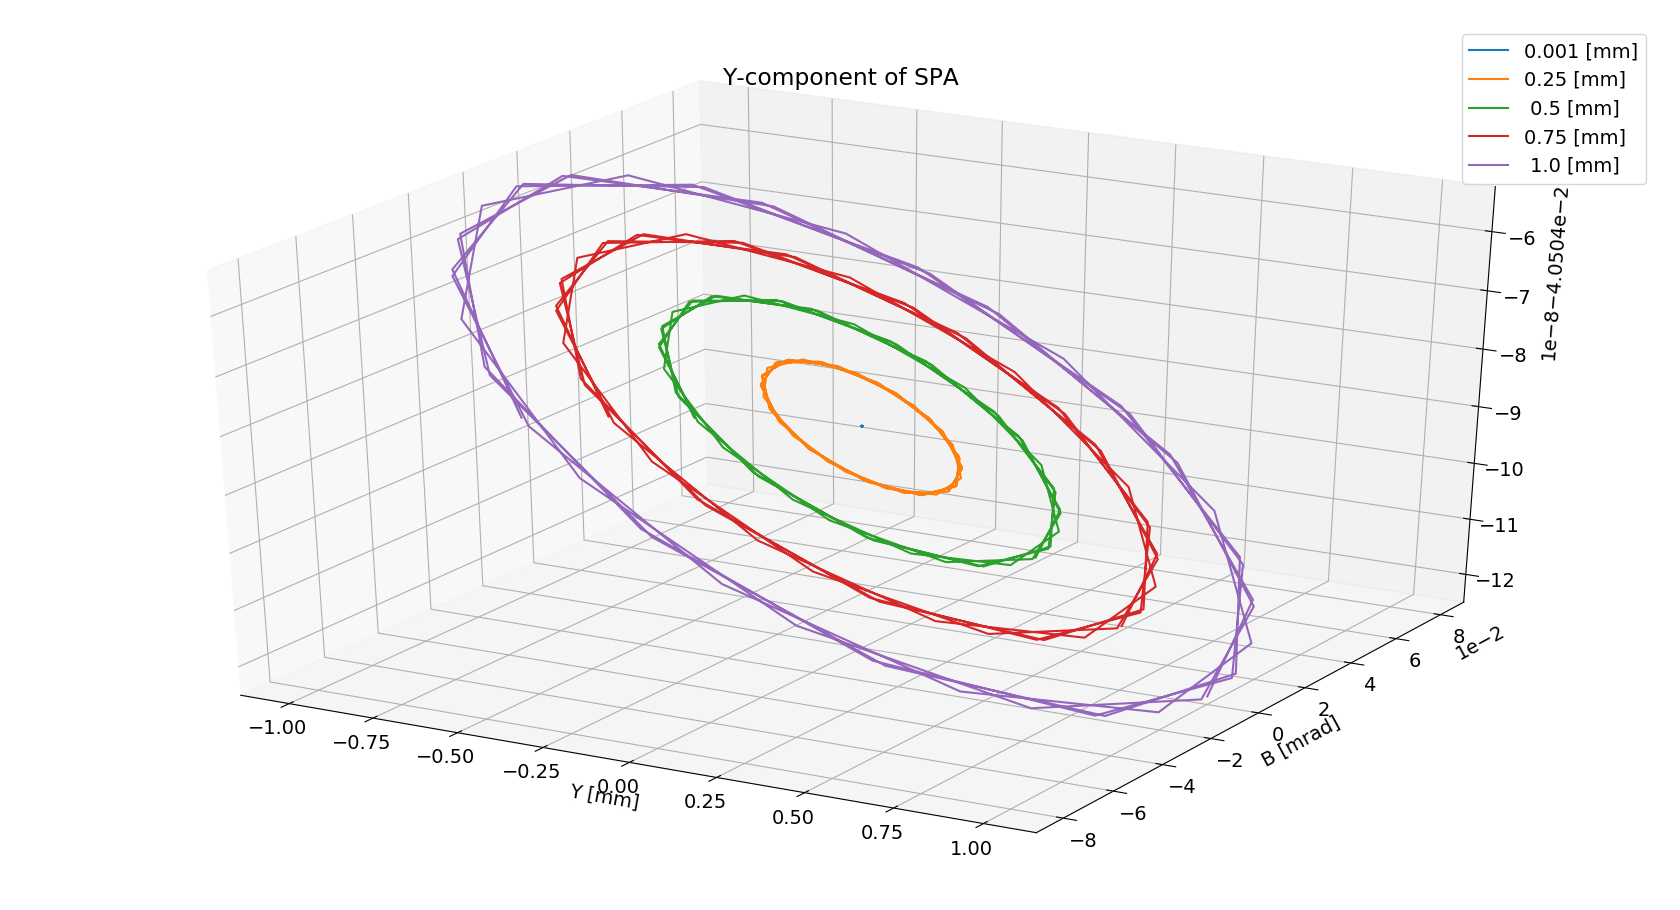
\includegraphics[width=\linewidth]{../img/IPAC19/NY_VS_YB_IMPERFECT_OPTIM}
    \caption{Используя секступоли\label{fig:spa_optim}}
  \end{subfigure}
  \caption{Вертикальная компонента инвариантной спиновой оси
    в имперфектной структуре как функция координаты фазового пространства $(y, y')$\label{fig:spa}}
\end{figure}

\paragraph{Классификация явлений}
Будем структурировать анализ спиновой динамики на основании геометрии функций спин-тюна и оси стабильного спина
от фазового пространства, рисунки~\ref{fig:spin_tune} и~\ref{fig:spa}.

Из этих рисунков можно наблюдать, что, во-первых, оба параметра являются фигурами вращения,
образованными \emph{параболой} (случай без секступолей), а во-вторых, фигура \emph{наклонена}
(это видно особенно отчётливо на рисунке~\ref{fig:spin_tune_optim}, где ещё видно параболу).
Таким образом, мы видим присутствие двух независимых явлений. Первое мы всегда называли спиновой декогкренцией,
а из-за второго происходит вариация спиновых параметров, вызванная бетатронным движением.
Его назовём SMP-эффектом.

(Отметим, что он существует в том числе и в идеальной структуре, и для всех фазовых плоскостей.)

\paragraph{Линейные эффекты декогеренции}
Во-первых, отмечу, что в диссере Еремея упоминаются ``линейные эффекты декогеренции,'' которые
минимизируются усреднением, путём использования ВЧ-поля. Очевидно то, что на рисунках выше, ВЧ-полем
не усреднится, но чисто структурно скорее всего это одно и то же. Я построил TSS-параметры
в зависимости от точек в плоскости $(\ell, \delta)$ для различных значений гармонического числа.
В случае успешной оптимизации, как и для других плоскостей, структура спин-тюна как на
рисунке~\ref{fig:tune_separatrix}. Когда мы увеличиваем гармоническое число, сжимается фазовый объём
пучка, и следовательно разброс спин-тюна. 


\begin{figure}[h]
  \centering
  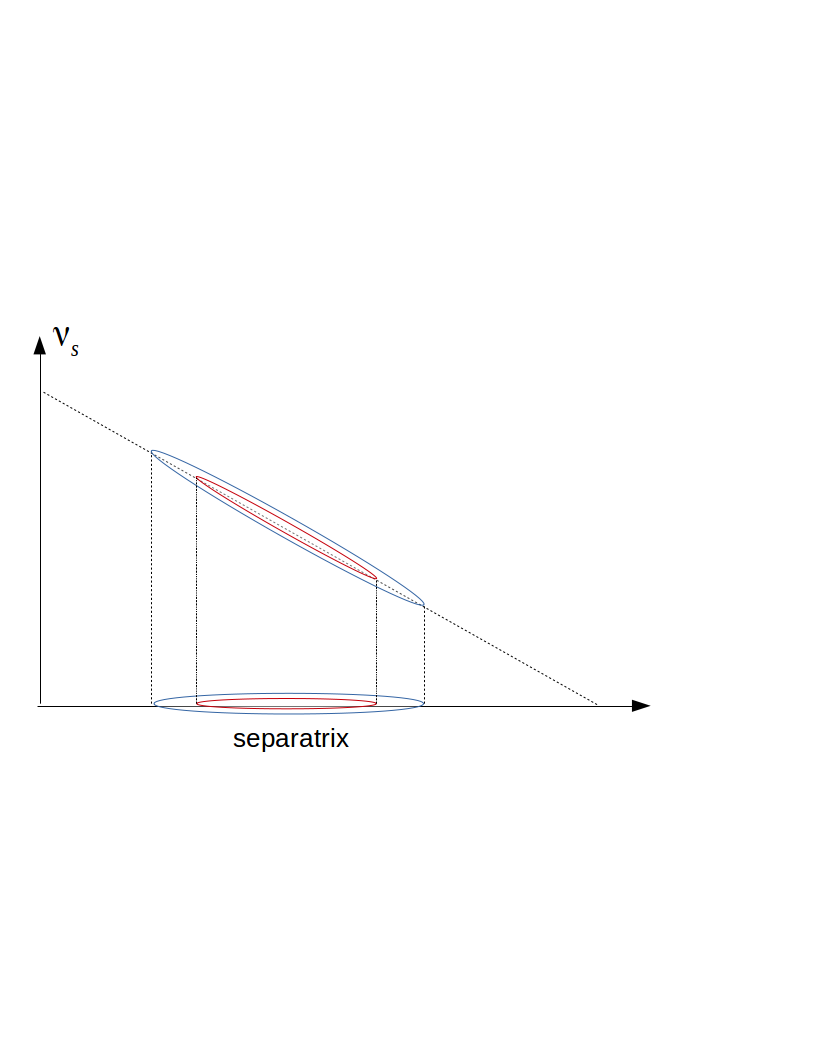
\includegraphics[width=\linewidth, trim=0 250 100 200, clip]{../img/IPAC19/tune_separatrix}
  \caption{Спин-тюн как функция фазового эллипса для двух банчей разного размера\label{fig:tune_separatrix}}
\end{figure}

\paragraph{Драфт основного рассмотрения SMP-эффекта}
Базовый посыл следующий:

Рассмотрим эволюцию вертикальной компоненты спина частицы:
\[
s_y(t) = \frac{\W_X}{\W}\sin(\W\cdot t + \phi_0).
\]

При этом, исходя из рисунков~\ref{fig:spin_tune_optim} и~\ref{fig:spa_optim}, в связи с бетатронным движением:
\begin{align}
  \W(t) &= \W_0 + a_1\sin(\W_1\cdot t + \phi_1), \tag{вариация спин-тюна}\\
  \W_X(t) &= \W(t)\cos\Theta(t), \tag{рисунок~\ref{fig:omega_plot}}\\
  \Theta(t) &= \Theta_0 + a_2\sin(\W_2\cdot t + \phi_2). \tag{вариация компонент $\bar n$}
\end{align}

\begin{figure}[h]
  \centering
  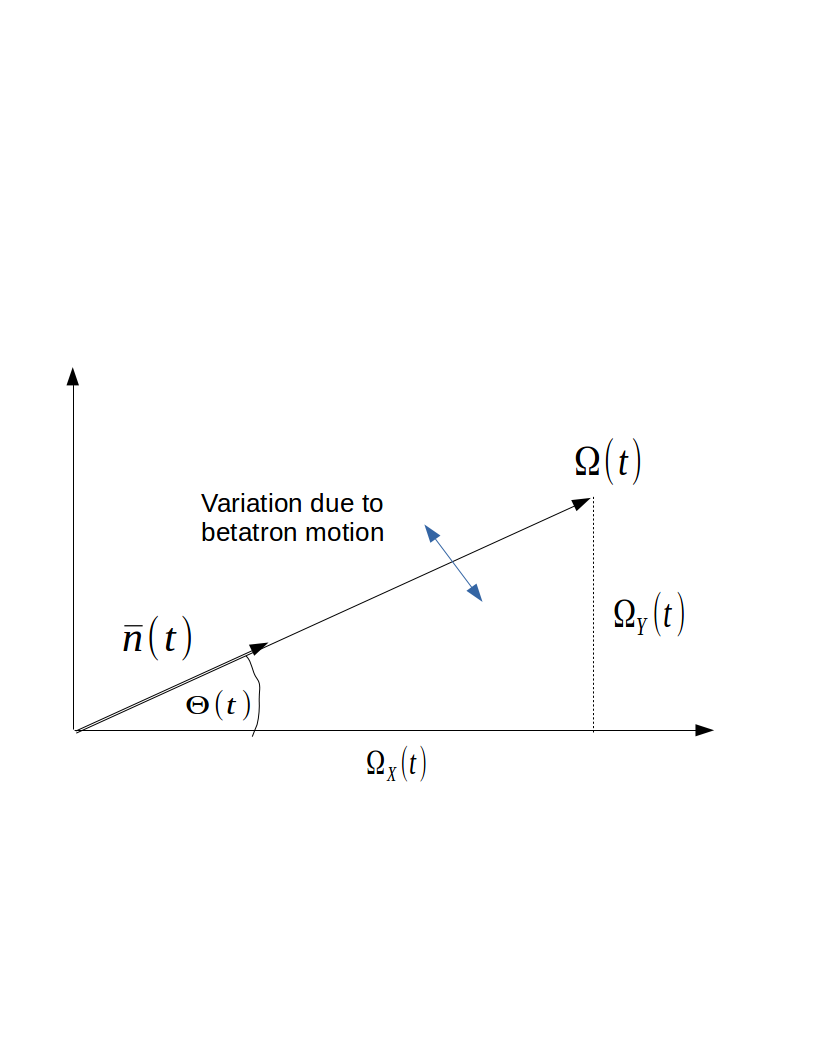
\includegraphics[width=\linewidth, trim=1 200 1 270, clip]{../img/IPAC19/omega_plot}
  \caption{Связь между компонентами частоты\label{fig:omega_plot}}
\end{figure}

Поскольку
\[
\frac{\W_X}{\W} = \frac{\W(t)\cos\Theta(t)}{\W(t)} = \cos\Theta(t),
\]
то
\[
s_y(t) = \cos\Theta(t)\cdot \sin\left(\W_0\cdot t + \phi_0 + a_1\sin\left[\W_1\cdot t + \phi_1\right]\cdot t\right)
\]

Чисто гипотетически, вот эту сложную функцию и надо фитировать. В ней учитывается вариация и магнитуды,
и направления спин-вектора Однако, по аналогии с энерго-зависимыми линейными эффектами декогеренции, можно
применить ту же логику, и сказать что данные эффекты усредняются. Если точнее, то они просто малы по сравнению
с другими ошибками. По крайней мере на это можно надеяться.

Как бы я проверил, посчитал средние значения для этой функции и для обычного синуса, и между ними невязка ---
растущая функция (значит частоты разные), но очень малой величины (оценки частот неразличимы, хотя простой
синус, конечно, фитируется намного точнее).

Возможно я неправильно оценил параметры возмущений частоты и амплитуды. Частота у меня варьируется с амплитудой
$5\cdot 10^{-10}$ от 50 рад/сек, а $\Theta$ с амплитудой $5\cdot 10^{-6}$ (разница между диапазоном
и оффсетом на оптимизированных рисунках), а частота бетатронных колебаний как для тюна 0.25.
 
\end{document}
